% =====================================================================
%  Colmeia de Morville Aplicada a 3 Softwares
%  Design Colaborativo - FEELT31623 - UFU - Prof. Renato Carrijo - 2026/2
%  Compilar com: latexmk -pdf -interaction=nonstopmode UX_final.tex
% =====================================================================
\documentclass[10pt,a4paper]{article}

\usepackage[T1]{fontenc}
\usepackage[utf8]{inputenc}
\IfFileExists{portuges.ldf}{\usepackage[brazil]{babel}}{}
\usepackage[scaled=0.92]{helvet}
\renewcommand{\familydefault}{\sfdefault}
\usepackage{microtype}

\usepackage[a4paper,top=2.4cm,bottom=2cm,left=2cm,right=2cm,headheight=28pt,headsep=14pt]{geometry}
\usepackage[table]{xcolor}
\usepackage{tabularx}
\usepackage{array}
\usepackage{fancyhdr}
\usepackage{tikz}
\usepackage[hidelinks]{hyperref}
\hypersetup{pdftitle={Colmeia de Morville Aplicada a 3 Softwares},
            pdfauthor={Prisma UX Design}}

% ---------------------------------------------------------------------
%  Paleta
% ---------------------------------------------------------------------
\definecolor{navy}{HTML}{1E3A8A}      % faixa das fichas / cabeçalho
\definecolor{navytext}{HTML}{1F2F5C}  % títulos
\definecolor{bodytext}{HTML}{374151}  % texto das células
\definecolor{labeltext}{HTML}{1F2937} % rótulos
\definecolor{gridline}{HTML}{9CA3AF}  % bordas das tabelas
\definecolor{secbg}{HTML}{E8EDF5}     % linha de seção
\definecolor{subtle}{HTML}{4B5563}    % subtítulo
\definecolor{cream}{HTML}{FFF8E1}     % fundo da melhoria
\definecolor{gold}{HTML}{D4A017}      % borda da melhoria
\definecolor{amber}{HTML}{B45309}     % rótulo da melhoria

% ---------------------------------------------------------------------
%  Cabeçalho e rodapé
% ---------------------------------------------------------------------
\pagestyle{fancy}
\fancyhf{}
\fancyhead[L]{\textcolor{navytext}{\bfseries\small DESIGN COLABORATIVO \textbullet\ FEELT31623}}
\fancyhead[R]{\footnotesize\color{subtle}%
  \begin{tabular}[b]{@{}r@{}}Universidade Federal de Uberlândia\\
  Prof. Renato Carrijo \textbullet\ 2026/2\end{tabular}}
\fancyfoot[C]{\footnotesize\color{subtle}\thepage}
\renewcommand{\headrulewidth}{0.8pt}
\renewcommand{\headrule}{{\color{navytext}\hrule height\headrulewidth width\headwidth}}

\setlength{\parindent}{0pt}
\setlength{\tabcolsep}{6pt}
\arrayrulecolor{gridline}

% ---------------------------------------------------------------------
%  Macros
% ---------------------------------------------------------------------
\newcolumntype{L}{>{\raggedright\arraybackslash\leavevmode\color{labeltext}}p{3.4cm}}
\newcolumntype{Y}{>{\raggedright\arraybackslash\leavevmode\color{bodytext}}X}

% Faixa azul do título da ficha
\newcommand{\ficha}[2]{%
  \par\vspace{4pt}\noindent
  \colorbox{navy}{\parbox{\dimexpr\linewidth-2\fboxsep\relax}{%
    \vspace{4pt}%
    \textcolor{white}{\bfseries #1}\hfill
    \textcolor{white}{\bfseries\itshape\small #2}%
    \vspace{4pt}}}%
  \par\vspace{8pt}}

% Linha simples (rótulo | conteúdo)
\newcommand{\linha}[2]{#1 & #2 \\ \hline}

% Nota de 1 a 5 em pontos (preenchidos em navy, vazios em cinza)
\newcommand{\nota}[1]{\tikz[baseline=-0.6ex]{\foreach \i in {1,...,5}{%
  \ifnum\i>#1\relax\def\notacor{gridline!60}\else\def\notacor{navy}\fi
  \fill[\notacor] (\i*6pt,0) circle (2.1pt);}}}

% Linha de faceta da Colmeia (rótulo + nota | conteúdo)
\newcommand{\faceta}[3]{\linha{#1\hfill\nota{#2}}{#3}}

% Linha de seção
\newcommand{\secao}[1]{%
  \multicolumn{2}{|>{\columncolor{secbg}}l|}{\textcolor{navytext}{\bfseries\footnotesize #1}} \\ \hline}

% Ambiente de tabela da ficha
\newenvironment{tabela}
  {\small\renewcommand{\arraystretch}{1.22}%
   \noindent\tabularx{\linewidth}{|L|Y|}\hline}
  {\endtabularx\par\vspace{7pt}}

% Caixa "Melhoria proposta"
\newcommand{\melhoria}[1]{%
  {\small\renewcommand{\arraystretch}{1.22}%
   \arrayrulecolor{gold}\setlength{\arrayrulewidth}{0.8pt}%
   \noindent
   \begin{tabularx}{\linewidth}{|>{\columncolor{cream}\raggedright\arraybackslash}p{3.4cm}|>{\columncolor{cream}\raggedright\arraybackslash\leavevmode\color{bodytext}}X|}
   \hline
   \textcolor{amber}{\bfseries Melhoria proposta} & #1 \\ \hline
   \end{tabularx}%
   \arrayrulecolor{gridline}}\par}

\newcommand{\metrica}{\textcolor{labeltext}{\bfseries Métrica sugerida:}}

% Favo hexagonal da Colmeia: {posição}{nota}{rótulo}
\newcommand{\favoR}{0.7cm}   % raio do hexágono
\newcommand{\favoD}{1.22cm}  % distância entre centros vizinhos
\newcommand{\favo}[3]{%
  \ifcase#2\relax
  \or\def\favocor{navy!15}\def\favotxt{navytext}%
  \or\def\favocor{navy!30}\def\favotxt{navytext}%
  \or\def\favocor{navy!50}\def\favotxt{navytext}%
  \or\def\favocor{navy!75}\def\favotxt{white}%
  \or\def\favocor{navy}\def\favotxt{white}\fi
  \begin{scope}[shift={#1}]
    \filldraw[fill=\favocor, draw=white, line width=1.2pt]
      (30:\favoR) -- (90:\favoR) -- (150:\favoR) -- (210:\favoR) -- (270:\favoR) -- (330:\favoR) -- cycle;
    \node[text=\favotxt, align=center, font=\fontsize{5}{6}\selectfont] at (0,0)
      {#3\\[1pt]{\fontsize{8}{9}\selectfont\bfseries #2}};
  \end{scope}}

% Colmeia completa (disposição de Morville, Valioso no centro):
% {x}{nome}{útil}{utilizável}{desejável}{encontrável}{acessível}{crível}{valioso}
\newcommand{\colmeia}[9]{%
  \begin{scope}[shift={(#1,0)}]
    \favo{(120:\favoD)}{#3}{Útil}
    \favo{(60:\favoD)}{#4}{Utilizável}
    \favo{(180:\favoD)}{#5}{Desejável}
    \favo{(0:\favoD)}{#6}{Encontrável}
    \favo{(240:\favoD)}{#7}{Acessível}
    \favo{(300:\favoD)}{#8}{Crível}
    \favo{(0,0)}{#9}{Valioso}
    \node[font=\small\bfseries, text=navytext, anchor=base] at (0,-2.2) {#2};
  \end{scope}}

% =====================================================================
\begin{document}

% ---------------------------------------------------------------------
%  Capa / identificação
% ---------------------------------------------------------------------
{\color{navytext}\fontsize{16}{20}\selectfont\bfseries Colmeia de Morville Aplicada a 3 Softwares\par}
\vspace{2pt}
{\color{subtle}\small Relatório de Avaliação da Experiência do Usuário (UX) e da Facilidade de Uso\par}
\vspace{8pt}

{\small\renewcommand{\arraystretch}{1.22}%
\noindent
\begin{tabularx}{\linewidth}{|>{\leavevmode\color{labeltext}}p{3.4cm}|>{\leavevmode\color{bodytext}}X|>{\leavevmode\color{labeltext}}p{3.2cm}|>{\leavevmode\color{bodytext}}X|}
\hline
Nome do Grupo & Prisma UX Design                & Líder do Grupo & Wilson Ribeiro de Andrade Filho \newline Matrícula: 12311ECP006 \\ \hline
Integrante 2  & José Mendes de Sousa \newline Matrícula: 12211ECP012 & Integrante 3 & José Lucas Lira \newline Matrícula: 12411ECP005 \\ \hline
Integrante 4  & Ana Flávia de Oliveira \newline Matrícula: 12411ECP025 & Integrante 5 & Emanuel Simões Campos \newline Matrícula: 12311ECP031 \\ \hline
\end{tabularx}\par}
\vspace{8pt}

% =====================================================================
%  FICHA 1 — DUOLINGO
% =====================================================================
\ficha{FICHA 1 --- SOFTWARE 1: DUOLINGO}{Análise de Aplicativo para Celular}

\begin{tabela}
\linha{Software escolhido}{\textbf{Duolingo} (aplicativo para celular)}
\linha{Tarefa}{Concluir uma lição diária de vocabulário básico.}
\linha{Persona}{Estudante iniciante no idioma, que estuda nos intervalos livres do dia e se motiva com pequenas conquistas.}
\linha{Contexto}{Celular na mão, no ônibus ou numa pausa do trabalho, com o som ligado ou desligado.}
\linha{Critério de sucesso}{Terminar a lição em menos de 5 minutos, sem perder a sequência de dias seguidos (ofensiva) e sem esgotar as vidas.}
\end{tabela}

\begin{tabela}
\secao{PRINCÍPIOS DE INTERAÇÃO E ERGONOMIA DIGITAL}
\linha{Lei de Fitts}{O botão ``Verificar/Continuar'' ocupa toda a largura da parte de baixo da tela, e as respostas são blocos grandes, fáceis de tocar.}
\linha{Lei de Hick}{Cada exercício mostra poucas alternativas por vez (em geral 3 ou 4), então a escolha é rápida.}
\linha{Thumb zones}{O botão ``Verificar'' fica fixo na parte de baixo da tela, onde o polegar alcança naturalmente.}
\linha{Microinteração}{Ao acertar, a faixa de baixo fica verde com uma mensagem de incentivo, um som de acerto e uma vibração curta.}
\linha{Tipografia}{Letras grandes e arredondadas (Feather Bold nos títulos e DIN Next Rounded no restante), com bom contraste entre os cartões e o fundo.}
\end{tabela}

\begin{tabela}
\secao{COLMEIA DA EXPERIÊNCIA DE MORVILLE (2004)}
\faceta{Útil}{3}{Ajuda a criar o hábito de estudar todo dia e a memorizar palavras básicas, mas explica pouco a gramática quando o usuário erra.}
\faceta{Utilizável}{4}{As perguntas de uma lição seguem em sequência, sem telas ou passos complicados no meio.}
\faceta{Desejável}{5}{Visual amigável, animações do mascote Duo e recompensas deixam o uso divertido e prendem a atenção.}
\faceta{Encontrável}{4}{A trilha de lições aparece logo na tela inicial, em ordem, sem que seja preciso procurá-la.}
\faceta{Acessível}{3}{Dá para pausar os exercícios de áudio e fala (``Não posso ouvir/falar agora''), o que ajuda em lugares barulhentos ou para quem tem dificuldade para ouvir ou falar.}
\faceta{Crível}{3}{Os cursos seguem os níveis do Quadro Europeu Comum de Referência para Línguas e mostram o progresso na hora; porém, às vezes uma tradução correta é marcada como errada.}
\faceta{Valioso}{4}{O usuário aprende de graça em sessões curtas; a empresa ganha com anúncios e assinaturas (Super e Max), graças ao uso diário.}
\end{tabela}

\melhoria{Mostrar, também no plano gratuito, uma explicação simples de gramática na própria tela de erro (hoje isso só existe no ``Explicar minha resposta'' do Duolingo Max e nas Dicas da unidade). Isso fortalece as facetas \textbf{Útil} e \textbf{Crível} e evita que o usuário aprenda só por tentativa e erro. \metrica{} quantas vezes o usuário acerta uma questão que já tinha errado antes, comparando um grupo que vê a explicação com outro que não vê (meta: 15 pontos percentuais a mais).}

\newpage
% =====================================================================
%  FICHA 2 — MIRO
% =====================================================================
\ficha{FICHA 2 --- SOFTWARE 2: MIRO}{Análise de Quadro Colaborativo no Computador}

\begin{tabela}
\linha{Software escolhido}{\textbf{Miro} (navegador e aplicativo para computador)}
\linha{Tarefa}{Organizar ideias em notas adesivas virtuais e ligá-las entre si, ao vivo, durante uma reunião.}
\linha{Persona}{Designer ou gerente de produto numa reunião on-line de troca de ideias (\textit{brainstorming}), usando o computador.}
\linha{Contexto}{Tela de computador, mouse ou \textit{trackpad} e teclado, com a chamada de vídeo aberta ao mesmo tempo.}
\linha{Critério de sucesso}{Organizar 5 ideias em notas e ligá-las em menos de 2 minutos, sem atrapalhar o andamento da reunião.}
\end{tabela}

\begin{tabela}
\secao{PRINCÍPIOS DE INTERAÇÃO E ERGONOMIA DIGITAL}
\linha{Lei de Fitts}{Os ícones da barra lateral de ferramentas são bem espaçados, mas os pontos usados para ligar setas entre as formas são pequenos e exigem mira precisa com o mouse.}
\linha{Lei de Hick}{Ao selecionar uma nota, aparece só uma pequena barra com as opções que fazem sentido (cor, tamanho e formato do texto, etiquetas, link e reações); o resto fica guardado no menu ``\ldots''.}
\linha{Thumb zones}{Não se aplica (uso no computador); no celular, os botões principais para inserir itens ficam na parte de baixo da tela.}
\linha{Microinteração}{Ao arrastar uma nota, aparecem linhas coloridas que ajudam a alinhá-la com as vizinhas; com a nota selecionada, botões ``+'' nas bordas criam uma nova nota já ligada à primeira.}
\linha{Tipografia}{O tamanho da letra se ajusta sozinho para o texto caber dentro da nota enquanto o usuário digita.}
\end{tabela}

\begin{tabela}
\secao{COLMEIA DA EXPERIÊNCIA DE MORVILLE (2004)}
\faceta{Útil}{5}{Reúne num só lugar as ideias de equipes que trabalham a distância.}
\faceta{Utilizável}{3}{Mover e ampliar o quadro é fácil e há atalhos de uma tecla (ex.: ``N'' cria uma nota), mas ligar setas entre notas exige mira precisa.}
\faceta{Desejável}{4}{Ver o cursor com o nome de cada colega, reações, cronômetro e votação deixa as dinâmicas em grupo mais animadas.}
\faceta{Encontrável}{3}{A busca (\texttt{Ctrl/Cmd+F}) e a lista de seções do quadro ajudam a achar conteúdo, mas quadros grandes ficam difíceis de percorrer.}
\faceta{Acessível}{2}{É difícil navegar pelo quadro, que não tem limites, usando só o teclado, sem o mouse.}
\faceta{Crível}{4}{Tudo é salvo e sincronizado na hora, sem perda de dados, mesmo com várias pessoas editando o mesmo trecho.}
\faceta{Valioso}{4}{Substitui o quadro físico e torna mais rápidas as reuniões de alinhamento e as dinâmicas em grupo.}
\end{tabela}

\melhoria{Aumentar a área dos pontos de ligação e mostrar uma prévia da seta quando o cursor se aproxima, fortalecendo a faceta \textbf{Utilizável} e reduzindo a mira exigida pela \textbf{Lei de Fitts}. \metrica{} tempo médio e número de tentativas erradas para ligar 5 notas, em teste com 5 participantes (meta: 30\% menos tempo).}

\newpage
% =====================================================================
%  FICHA 3 — SPOTIFY
% =====================================================================
\ficha{FICHA 3 --- SOFTWARE 3: SPOTIFY}{Análise de Aplicativo de Música}

\begin{tabela}
\linha{Software escolhido}{\textbf{Spotify} (aplicativo para celular)}
\linha{Tarefa}{Buscar uma playlist de músicas para treino, salvar uma música na biblioteca e começar a ouvir.}
\linha{Persona}{Pessoa que ouve música no celular enquanto se desloca ou treina na academia, com o app em segundo plano.}
\linha{Contexto}{Celular com fones de ouvido sem fio, usando internet móvel (4G/5G).}
\linha{Critério de sucesso}{Concluir a tarefa em até 30 segundos e com no máximo 6 toques, sem contar a digitação da busca.}
\end{tabela}

\begin{tabela}
\secao{PRINCÍPIOS DE INTERAÇÃO E ERGONOMIA DIGITAL}
\linha{Lei de Fitts}{O botão verde de tocar, na página da playlist, é grande e fica separado dos demais; no mini-player da parte de baixo, o botão de tocar/pausar é fácil de acertar sem olhar com atenção.}
\linha{Lei de Hick}{Botões de filtro no topo da tela inicial (Tudo, Música, Podcasts) reduzem o que aparece de uma vez, e cada seção mostra poucos itens por linha.}
\linha{Thumb zones}{O mini-player e o menu principal (Início, Buscar, Sua Biblioteca) ficam na parte de baixo da tela, fáceis de alcançar com o polegar.}
\linha{Microinteração}{Ao tocar no ``+'' de uma música, ele vira um sinal de confirmação verde e aparece um aviso rápido de que ela foi salva nas Músicas Curtidas.}
\linha{Tipografia}{Fonte própria do Spotify (Spotify Mix, desde 2024), em negrito nos títulos de álbuns e playlists, bem legível sobre o fundo escuro.}
\end{tabela}

\begin{tabela}
\secao{COLMEIA DA EXPERIÊNCIA DE MORVILLE (2004)}
\faceta{Útil}{5}{Dá acesso imediato a um enorme acervo de músicas e podcasts.}
\faceta{Utilizável}{3}{A música continua tocando enquanto se navega pelo app, mas salvar uma faixa da lista exige acertar um ícone pequeno ou abrir o menu ``\ldots''.}
\faceta{Desejável}{5}{Vídeos curtos no fundo das músicas (Canvas) e playlists personalizadas criam uma ligação afetiva com o app.}
\faceta{Encontrável}{5}{A busca é rápida, completa o texto enquanto se digita e permite filtrar por artista, música ou álbum.}
\faceta{Acessível}{3}{Funciona com os leitores de tela do celular (VoiceOver/TalkBack) e mostra letras sincronizadas, que ajudam pessoas surdas ou com perda auditiva; mas alguns botões são pequenos.}
\faceta{Crível}{4}{A música não para ao trocar de faixa, e os downloads para ouvir sem internet mantêm o som estável mesmo com sinal fraco.}
\faceta{Valioso}{4}{Oferece uma grande biblioteca e recomendações feitas sob medida, em troca da assinatura ou de anúncios.}
\end{tabela}

\melhoria{Deixar o usuário escolher o que acontece ao deslizar uma música para o lado (hoje ela só vai para a fila), podendo usar esse gesto para salvá-la na biblioteca. Isso dispensa o menu extra e fortalece a faceta \textbf{Utilizável}; pela \textbf{Lei de Fitts}, a área de toque passa a ser a linha inteira. \metrica{} toques e tempo para salvar 3 músicas na biblioteca (meta: de cerca de 9 para 3 toques), em teste com 5 usuários.}

\newpage
% =====================================================================
%  SÍNTESE COMPARATIVA
% =====================================================================
\ficha{SÍNTESE COMPARATIVA}{Colmeia de Morville nos 3 softwares}

{\small\color{bodytext}Cada favo mostra a nota de 1 (fraco) a 5 (excelente) que o grupo deu à faceta, com base no que foi observado nas fichas; quanto mais escuro o favo, maior a nota.\par}
\vspace{12pt}

\begin{center}
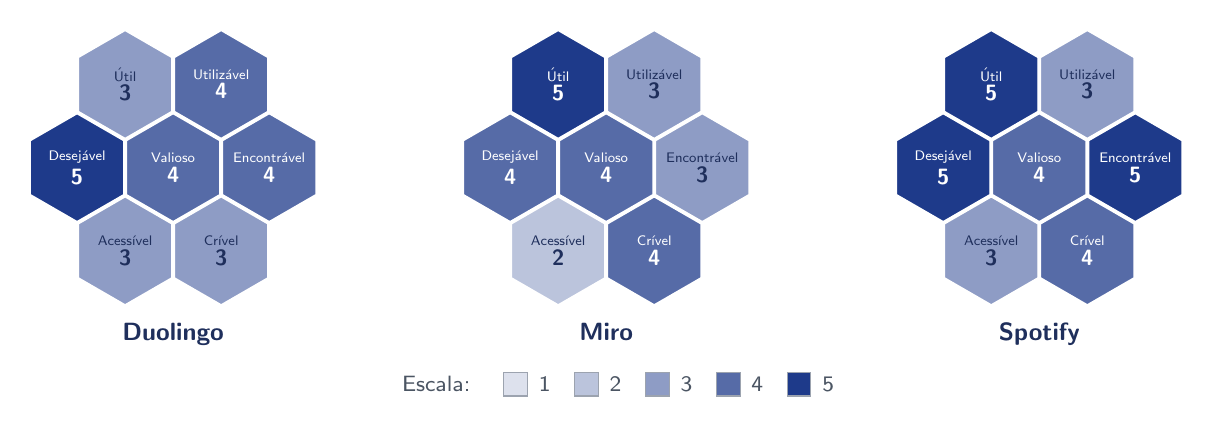
\begin{tikzpicture}
  \colmeia{0}{Duolingo}{3}{4}{5}{4}{3}{3}{4}
  \colmeia{5.5}{Miro}{5}{3}{4}{3}{2}{4}{4}
  \colmeia{11}{Spotify}{5}{3}{5}{5}{3}{4}{4}
  % Legenda da escala
  \node[font=\footnotesize, text=subtle, anchor=east] at (3.9,-2.75) {Escala:};
  \foreach \n/\c in {1/navy!15, 2/navy!30, 3/navy!50, 4/navy!75, 5/navy} {
    \filldraw[fill=\c, draw=gridline, line width=0.4pt]
      ({3.9+0.9*\n-0.6},-2.9) rectangle ++(0.3,0.3);
    \node[font=\footnotesize, text=subtle, anchor=west] at ({3.9+0.9*\n-0.28},-2.75) {\n};
  }
\end{tikzpicture}
\end{center}
\vspace{4pt}

{\small\renewcommand{\arraystretch}{1.22}%
\noindent
\begin{tabularx}{\linewidth}{|Y|}
\hline
\rowcolor{secbg}\textcolor{navytext}{\bfseries\footnotesize CONCLUSÃO} \\ \hline
O Spotify foi o mais bem avaliado dos três, e \textbf{Desejável} foi o ponto mais forte do conjunto: os três aplicativos se esforçam para tornar o uso agradável e trazem benefícios tanto para quem usa quanto para a empresa. Já \textbf{Acessível} foi o ponto mais fraco, principalmente no Miro, cujo quadro sem limites é difícil de usar com leitores de tela ou só com o teclado. As melhorias propostas atacam os pontos mais fracos de cada ficha e trazem uma forma simples de medir se funcionaram. \\ \hline
\end{tabularx}\par}

\end{document}
